\chapter{System Design}
Laha, which means, to spread or distribute in Hawaiian, is an abstract framework for distributed sensor networks that provides a means for turning primitive data into actionable insights, tiered management of voluminous amounts of sensor data. This major goals are in part accomplished by augmenting a DSN with the ability to adaptively optimize its bandwidth, detection, classification, and sensor device power requirements.

The Laha framework is made up of five levels that can be viewed conceptually as a pyramid (see \ref{laha-figure}). Primitive data entering the Laha framework is located at the bottom the bottom of the pyramid. As data moves upward through the levels, noise is discarded, less interesting events are discarded or aggregated into upper levels, events are given more meaning and context, and associations and predictions are made. 

\begin{figure}
\caption{Laha Conceptual Model}
\centering
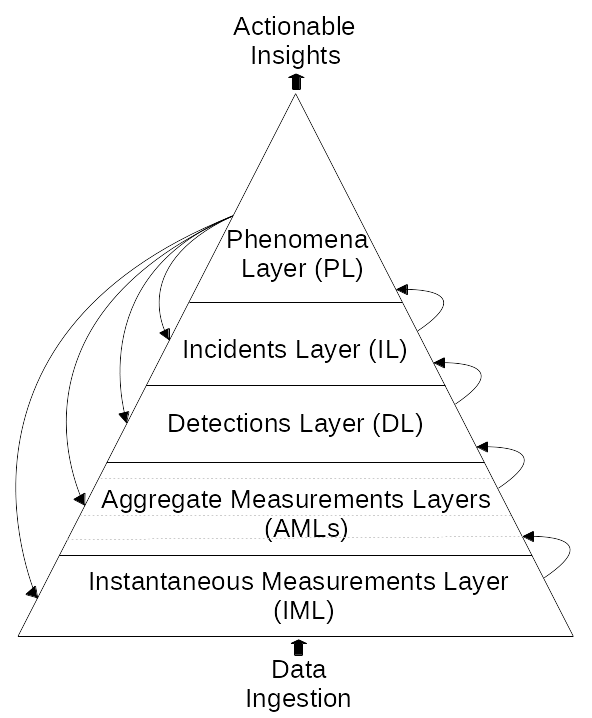
\includegraphics{figures/laha.png}	
\label{laha-figure}
\end{figure}

%\section{Five proposed benefits of Laha} \label{laha-benefits}
%Laha is designed to adaptively optimize the collection, triggering, detection, and classification of signals within a DSN. These optimizations provide several benefits to DSNs. Many of these benefits can be found in other DSNs, but generally only appear as a single optimization (TODO: CITE) or as a subset of optimizations (TODO: CITE). Laha is the first DSN to combine all of these benefits for the purpose of auto-optimizing the network.

%\subsection{Tiered management of Big Data}
%% TODO If you're going to use "Big Data" as a term of art, then it needs to be rigorously defined.
%% TODO What I think you need to emphasize here is that in any Big Data scenario, you simply can't keep all the data around forever. So, what approach will be used to decide what data to keep and what data to discard?  Laha addresses this problem by having a series of levels, each with its own TTL.  This approach has the benefit of simplifying the analysis of bandwidth and storage requirements for a DSN, but at the cost of potentially discarding important data due to the "use it or lose it" design.  Part of youer evaluation should attempt to address this weakness of use it or lose it.
%
%Laha provides tiered management of the Big Data that the framework consumes. This is mainly accomplished using the layered approach that Laha provides. All data within the Laha framework is garbage collected using a configurable time to live (TTL) for each level. As data moves from the bottom to the top of the framework, noise is discarded and only interesting data as determined by the higher levels is preserved and forwarded upwards within the framework. In this way, the network can be tuned to preserve increasingly important data. One of the drawbacks of this approach is that it's possible to accidentally discard data that does contain signals of interest, but were not detectable using the current set of detection and classification algorithms. Not only does tiered management of big data increase the signal-to-noise ratio as data is moved upwards, but it also provides graceful degradation so that data pressure is never a reason a DSN is brought down. The TTL for each level can be tuned by Laha's Phenomena to either optimize for system performance or to optimize for signal analysis The details of Laha's tiered approach can be found in section \ref{big-data-management}.
%
%\subsection{Automatically provide context to classified incidents}
%% TODO This is a feature that will be hopefully much more easily evaluated once you have the two reference implementations.  I will be interested to see what kinds of contextual information are attached, and whether there are times you wished you could attach information elsewhere.
%Laha provides Annotations Phenomena (see \ref{annotations-phenomena}) that allows users or algorithms to tag signals of interest with contextual information. There is already a large amount of research for providing classifications of signals of interest, however annotations provide context about the classifications themselves. That is, Laha provides the ability to assign causality to already classified signals.
%
%Initially, a library of annotations is required to be built for a particular DSN. Once the library has been built, Laha can provide automatic annotation assignment using similarity metrics. By using annotations and determining causality, it's possible to create actionable responses to signals observed within a network.
%
%Further, annotations can be used to optimize detection and classification of known signals. For example, imagine a power quality network that observes a voltage sag on the same sensors at the same time periodically. If the cause of the voltage sag can be determined (such as a motor turning on), then detection of this signal can either be muted or analyzed more deeply. Also, other voltage sags that exhibit similar characteristics can then be automatically annotated.
%
%\subsection{Adaptive optimizations for triggering}
%% TODO This seems totally cool, but I question whether this is a novel feature. Adaptive setting of thresholds must happen in lots of different domains.  You'll want to discuss related work here, and hopefully argue that other approaches are ad-hoc and domain-specific, but the contribution of Laha is to build adaptive optimization of triggering directly into the framework as a first-class concept. 
%Many triggering schemes rely on thresholds being surpassed within feature extracted data streams. For example, triggered data streams in a power quality network might consist of voltage, frequency, and THD extracted features to determine if there is likely a signal of interest observed from a given set of sensors. If any of the extracted features surpass a preset threshold, then we end up triggering the devices for raw, higher fidelity data. However, there are cases where the feature extracted stream may not surpass a predefined threshold and those sensors would not be triggered.
%
%By using different types of Phenomena, I can improve our triggering efficiency. For example, Locality Phenomena, as discussed in section \ref{locality-phenomena}, allow us to predict detections and classifications in space. If a particular grouping of sensors that are related in space always observe the same detections and classifications, then I can build a predictive model of when the framework can expect to see those things. In this way, a sensor may trigger on a passed threshold, but other sensors that are co-located may not trigger because feature extracted data is below the triggering threshold. If the Locality Phenomena predicts that other co-located sensors should have detected the same signal, then Laha might trigger those devices for high fidelity data to determine if the signal is in the raw data stream even though it didn't meet the triggering threshold.
%
%Laha can use Periodicity Phenomena, as discussed in section \ref{periodicity-phenomena}, in similar ways. When periodic signals are classified, Laha can create Future Phenomena that predicts when signals of interest should be detected and classified. This allows Laha to optimize triggering by tuning the triggers to specifically look for Periodic or Future Phenomena. Periodic and Future Phenomena also allows Laha to tune classification algorithms to the predicted classifications.
%
%\subsection{Adaptive optimizations for detection and classification}
%Not only can Laha optimize triggering, but similar usages of Locality and Future phenomena can be utilized to improve detection and classification efficiency. With Locality Phenomena, a model of common detections and classifications can be built for a set of co-located sensors. Detection and classification algorithms can be tuned to search for specific signals that are often observed within this model, pruning the search space and increasing the accuracy of detection and classification algorithms.
%
%Future and Periodic Phenomena provide the same benefits to detection and classification as Locality Phenomena. That is, if Laha is able to predict when a signal is going to arrive and also predict how that signal is going to be classified, then it can tune its detection and classification algorithms specifically for the signal of interest.
%
%\subsection{Provides a model of underlying sensor field topology}
%% TODO Either this is extremely cool, or totally frivolous, and I'm not sure which. it is frivolous if the only thing it's doing is detecting topology that you already know about (i.e. that two OPQ boxes are close together physically, but we already know that because of their lat/long coordinates.) it is totally cool if you are detecting topology that is not already known. So, it would be good to provide a specific example here for both domains (OPQ and Lokahi)
%
%Predictive phenomena use localization of signals to build communities or groupings of sensors that observe similar signals in both time and space. Over time, Laha can begin to build a model of the underlying topology of the sensing field. For instance, if a group of sensors always see the same signal, then we can assume that either the signal has a far reach, or the sensors are grouped together geographically. With enough sensor penetration, we can differentiate between these two scenarios.
%
%Further, if the sensors provide any sort of location information, Laha can provide a mapping from physical location to sensor field topology. This is especially useful when the topology of the sensor field is not known a priori. Even if we know the location of the sensors at all times, that does not mean that we understand the topology of the sensing field. For example, in a PQ network, the topology is defined by how the electrical grid is connected to itself and laid out. Laha hopes to provide a model that can determine the electrical distance between devices even if the topology of the grid is not known. As another example, take an infrasound network. It's possible that two sensors are located close to each other geographically, but if they have a large mass between them, they may not receive the same signals due to the topology of the environment around them. 
%
%In this sense, Laha is not interested in knowing the location of sensors relative to each other, but is more interested in understanding how signals flow between sensors as a constraint on the topology that the signals travel through. That is, can Laha determine the statistical signal distance between sensors? And if it can, can the model be used to further tune lower levels of the Laha hierarchy?
%
%The aim is that if Laha can accurately provide a model of the underlying sensing field topology, this information can be used to optimize lower levels of the Laha hierarchy. For example, Laha can prime sensors for receiving or ignoring signals of interest by determining that a signal is supposed to arrive at a sensor before it does, i.e. Predictive Phenomena.

\section{Big Data Management in Laha} \label{big-data-management}
The Laha framework acts as an adaptive sieve for filtering noise and uninteresting data collected from a DSN. In this way, each level only passes what it considers interesting to the level above it. All data at a particular level is garbage collected at specific intervals relating to its important to the DSN.

Each level only keeps data for a specified amount of time before it is garbage collected. As data moves up the pyramid, it is generally considered more useful and therefore has a longer Time to Live (TTL), the amount of the time the data lives before it is garbage collected.  When a higher level detects ``something interesting", the data contained in the time window of ``something interesting" is copied into the levels above it and will still persist even though the original data is garbage collected. In this way, Laha preserves data from all levels if they are associated with interesting data. This also provides graceful degradation of services. The TTL is managed by the overall memory management of the system. Laha Actors are designed to work within the constraints of the TTL at different levels. If a constraint is broken, the Actor logs this issue. TTL can be optimized by Phenomena at each level to either tune for system performance or tune for decreasing of false positives and false negatives at different levels within the Laha hierarchy.

A summary of how data management in Laha is provided in table \ref{data-managament-table}. Note that the TTL is configurable for each implementing network and the table provides default values.

\begin{table}
	\caption{Summary of data management and context addition in Laha}
	\begin{tabular}{|c|c|c|}
		\hline 
		Level & Description & Time-to-Live (TTL) \\ 
		\hline 
		Phenomena Level (PL) & Contextual \& predictive analytics &  \\ 
		\hline 
		Incidents Level (IL) & Classified signals &  1 year \\ 
		\hline 
		Detections Level (DL) & Triggered windowed raw data & 1 week  \\ 
		\hline 
		Aggregate Measurements Level (AML) & Statistical aggregates of raw data  & 1 day  \\ 
		\hline 
		Instantaneous Measurements Level (IML) & Raw sensor data  & 1 hour \\ 
		\hline 
	\end{tabular} 
    \label{data-managament-table}
\end{table}

\subsection{Instantaneous Measurements Level}
The Instantaneous Measurements Level (IML) receives raw, sampled data from the DSN. The amount of data received is determined by the sample rate of each device multiplied by the number of fields per sample. Most of the time samples, from devices in the network are mainly sampling noise. A large percentage of the data in this level is destined for garbage collection and data is assigned a Time to Live (TTL) of one hour. 

\subsection{Aggregate Measurements Level}
The Aggregate Measurements Level (AML) is responsible for rolling up IMs from the IML. In general, this level only works with feature extracted data, rather than working with the raw samples. Each measurement in the AML provides summary statistics over a configurable time window. For example, these can include min, max, mean, median, mode, and variance statistics. 

It's possible to breakup the AML into several sub levels, each with different window sizes. For example, Laha might roll IMs into one minute AMs, then roll one minute AMs into hour AMs, then days, and so on. Each sublevel within the AML can have its own configurable TTL, ensuring long term summary statistics stick around for as long as needed. This provides us a high level view of the network and can provide insights into long term trends which wouldn't be visible (or available) in the IM data stream.

Similar to IMs, AMs can be saved and copied to the levels above it when interesting data is observed. This ability allows for AMs during these time periods to be stored and saved from the garbage collection process.

At this point in the hierarchy, we are still not providing any context to the data that we are receiving. Context is provided by levels above the AML.

\subsection{Detections Level}
The Detections Level (DL) is the first level that provides some context to the data that the sink is receiving. This level is responsible watching the feature extracted data streams, and requesting IMs from the IM level. In general, the detection level is meant to be trigger happy\footnote{Pun intended.} and be overly aggressive when determining if a feature extracted data stream looks interesting. 

When a data stream looks interesting, the DL marks a timestamp $N$ seconds before the interesting features and $M$ seconds after the interesting features, where both $N$ and $M$ are configurable within the framework. The goal is to use a time window that catches signals of interest within it. Since these data ranges will be further processed and refined higher in the hierarchy, there is no issue with collecting larges amounts of data in this level. 

The actual methods of detection is dependent on the characteristics of every individual sensor network. This framework assumes that the detection algorithms are provided by the implementing frameworks.

Similar to other levels, the DL level will have its IMs and AMs copied into levels above it when upper levels observe something interesting in the DL. The detections level is set to have a TTL of a week.

\subsection{Incidents Level}
Incidents represent classified signals. Incidents are individual classifications for signals of interest and are created by analyzing waveforms from Events. Waveforms from Events may contain multiple incidents. Individual signals may be classified as multiple incidents (for example a transient being classified as both a transient and frequency incidents). 

Incidents are further analyzed to produce phenomena. 

Incidents are expired after one year of storage. 


\subsection{Phenomena Level}
Phenomena are defined as a grouping of incidents that provide one or more of annotations, locality, periodicity, predictiveness, similarity, and future phenomena. 

Not only do Phenomena provide interesting insight and analytics into the underlying data, but they also provide a means for adaptively tuning the underlying collection, triggering, detection, and analysis of a distributed sensor network.

Phenomena are summarized in table \ref{phenomena-summary-table} and discussed in great detail in section \ref{phenomena}.

\section{Phenomena: Providing Adaptive Optimizations in Laha} \label{phenomena}

\begin{table}
	\centering
	\caption{Summary of Laha Phenomena}
	\begin{tabular}{|c|c|}
		\hline
		Phenomena & Description \\
		\hline
		Annotations & Provide context about an Incident or set of incidents \\
		\hline
		Locality & Provides context on how incidents are related in time and space \\
		\hline
		Periodicity & Designation for incidents that exhibit repetitive or periodic behavior \\ 
		\hline
		Similarity & Subset of incidents found using grouping and community detection algorithms \\
		\hline
		Predictive & Subset of incidents characterized by predictive or forecasting models\\
		\hline
		Future & Incidents scheduled to occur in the future\\
		\hline
	\end{tabular}
	\label{phenomena-summary-table}
\end{table}

\subsection{Annotations Phenomena} \label{annotations-phenomena}
Annotations provide context about an Incident or a set of Incidents. Annotations are generally user provided or sourced from other data sources to provide supporting context to Incidents. For example, Annotations might include “Cloud Cover”, “Hurricane Hector”, “Dryer Turns On”, etc.

In some sense, annotations allow us to label our data sets beyond a simple classification and start looking at causal classifications. Once enough annotations have been assigned to classified incidents, Laha can used Annotations to attempt to label unknown incidents with similar characteristics.

Annotations can be used to tune Laha's detection and classification algorithms by allowing Laha to filter on incidents with known causes.

\subsection{Locality Phenomena} \label{locality-phenomena}
Locality provides context on how incidents are related to each other in both space in time. Laha is able to determine if classified incidents are local to a single sensor, to a group of co-located sensors, or global across an entire network. Sensors can be co-located in both the physical sense and also co-located within a sensing field. For example, sensors in a power quality network may be separated by large distance geographically, but co-located through the electrical grid and the grid's topology. 

Over time, Locality Phenomena is used to build a model of sensors in relation to each other and to provide a statistical likelihood that co-located sensors will observe the same signal. Locality phenomena can be used to drive network triggering, detection, and classification thresholds within a distributed sensor network by using this probabilistic model for determining the likelihood that a sensor or sensors will observe a signal of interest.

\subsection{Periodicity Phenomena} \label{periodicity-phenomena}
Periodic phenomena consists of incidents that exhibit repetitive behavior, that is, the same types of incidents appearing in cycles from single or multiple devices. Periodicity allows for the easy creation of Predictive phenomena.

Periodic phenomena can come from a single incident or from multiple incidents. Periodic phenomena allow us to either tune our network to find periodic incidents or tune the  network to ignore periodic incidents depending on if the incidents are of interest. Periodic phenomena are especially useful in conjunction with Annotation phenomena as Laha can assign causality to the periodic signal. 

\subsection{Similarity Phenomena}
Similarity phenomena utilize grouping and community detection algorithms to group incidents together by their features. Common features used for grouping include time, location, incident type, or incident features.

\subsection{Predictive Phenomena}
Predictive phenomena consists of incidents that are characterized by a predictive or forecasting models. Predictiveness is a behavior that can be inferred from all other phenomena types. 

Predictiveness is the main driver behind optimizing the control of a distributed sensor network. If Laha can predict the types of signals that will arrive at sensors, then Laha can tune those sensors and the sink to either filter the signals (if the user is not interested in signals) or tune the sensors and the sink to be extra sensitive to those signals, possible detecting them even if they previously would not have been detected.

\subsection{Future Phenomena}
Predictive phenomena can be used to create future phenomena. Future phenomena are a statistical model of the likelihood of seeing an incident or incidents at future points in time. Knowing that a signal may occur with some probability allows Actor affected by those signals time to prepare for the signals.

\section{Laha Actors: Acting on the Laha Data Model}
Laha Actors act on the Laha hierarchy and provide one of two functions. Actors can move data from one level of the hierarchy upwards through the hierarchy when interesting data is requested by an upper level. Actors can also apply adaptive optimizations downwards through the hierarchy. The Laha framework can support multiple actors at each level. For example, the Incidents Level in our reference power quality network contains actors for each of the following functions: IEEE classified voltage events, frequency variations, power outages, excessive THD, and many others. The Incident Level Actors move data from these incidents upwards to the Phenomena Level.  

Table \ref{laha-actors-tables} summarizes the actors that exist within the Laha framework and their purposes. 

\begin{table}
	\centering
	\caption{Summary of Laha Actors}
	\begin{tabular}{|c|c|}
		\hline
		Actor & Purpose \\
		\hline
		IML Actors & Perform feature extraction and move aggregate data to AML \\
		\hline
		AML Actors & Perform triggering on data from IML, copy data to DL if interesting \\
		\hline
		DL Actors & Perform high fidelity feature extraction on possible detections \\
		\hline
		IL Actors & Perform classification and contextualization on possible detections \\
		\hline
		PL Actors & Generate predictive analytics and optimize the lower levels of the hierarchy \\
		\hline
	\end{tabular}
	\label{laha-actors-tables}
\end{table}

\subsection{Actor Constraints}
Actors at each level in the hierarchy are governed by a set of constraints. These constraints include the set of possible inputs, $A_i$, the set of possible outputs, $A_o$, the set of Actors it can receive data from, $A_{ai}$, the set of Actors it can transmit data to, $A_{ao}$, and a set of performance metrics that each actor must maintain, $A_p$. The constraints assigned to each Actor are determined by the hierarchy level in which the Actor resides.  

Actors are responsible for reporting constraint violations and in this way, Actors are the primary provider of health, performance, and status metrics about the Laha framework.

The constraints for each level of Laha hierarchy is summarized in table \ref{actor-constraint-table}.

\begin{table}
	\centering
	\caption{Summary of Laha Actor Constraints at Each Level}
	\begin{tabular}{|c|c|c|c|c|c|}
		\hline
		Level & $A_i$ & $Ao$ & $A_{ai}$ & $A_{ao}$ & $A_p$ \\
		\hline
		IML & Raw samples & Aggregate trends & n/a & AML & Data ranges available \\
		\hline
		AML & Aggregate trends & Detections & IML & DL & Data ranges available \\
		\hline
		DL & Windowed waveforms & Hi-fi extracted features & AML & IL & Data \& features available \\
		\hline
		IL & Hi-fi extracted features & Contextualized incidents & DL & PL & Incident types available \\
		\hline
		PL & Contextualized incidents & Optimizations & IL & All levels & Optimizations available \\
		\hline
	\end{tabular}
	\label{actor-constraint-table}
\end{table}

\section{OPQ: A Laha-compliant Power Quality DSN}
OPQMauka is a middleware component of the Open Power Quality (OPQ) framework. The OPQ project provides a hardware and software solution for monitoring distributed power quality (PQ). The OPQ project was founded with the goal of studying how intermittent distributed renewable energy sources affect PQ not just at a user's home, but also within a user's neighborhood, between neighborhoods, and globally across the grid. 

The OPQ ecosystem is made up of networked hardware sensors (OPQBoxes) and various software services (OPQMakai, OPQMauka OPQHealth, OPQView). Each of these software components are made up of individual services and plugins. The entire software system is deployed as Docker containers.

The OPQ system design is laid out in figure \ref{fig:opq-system}.

\begin{figure}
	\centering
	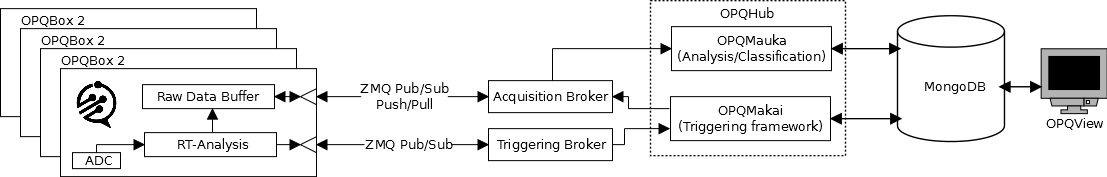
\includegraphics[width=\linewidth]{figures/system-diagram.png}
	\caption{OPQ System Diagram}\label{fig:opq-system}
\end{figure}


\subsection{OPQ: Boxes}
An OPQ Box is a custom designed PQ sensor. OPQBoxes can be plugged into a wall outlet and communicate with OPQ servers using the user's WiFi connection. OPQBoxes consist of a Raspberry PI single board computer (SBC), a custom board for PQ measurements, custom firmware, and a custom enclosure. The custom board contains an ADC that samples an alternating current (AC) power signal at 12 thousand samples per second. This data is transferred to the Raspberry Pi where feature extraction and data transfer takes place. The hardware design is presented in figure \ref{fig:opq-box-design} and the software design is provided in figure \ref{}.

\begin{figure}
	\centering
	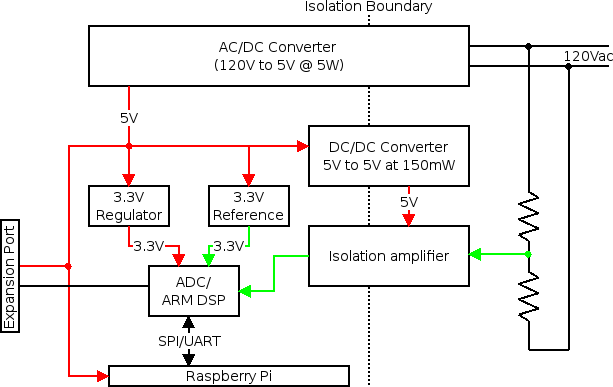
\includegraphics[width=.75\linewidth]{figures/opqbox_diagram.png}
	\caption{OPQ Box Design}\label{fig:opq-box-design}
\end{figure}

\begin{figure}
	\centering
	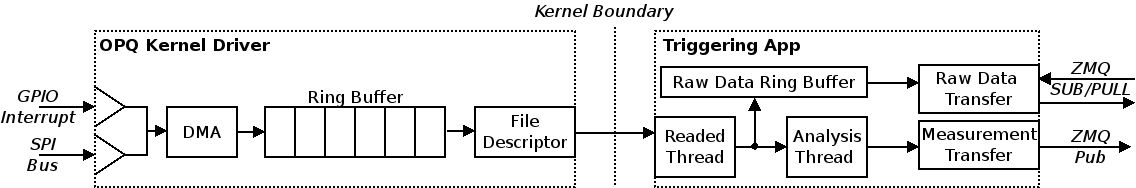
\includegraphics[width=.75\linewidth]{figures/opqbox_software.png}
	\caption{OPQ Box Software}\label{fig:opq-box-software}
\end{figure}

The feature extraction algorithms extract from the sampled waveform the following features: windowed $V_{RMS}$, frequency, and total harmonic distortion (THD) features. The feature extracted data is then sent to a central sink where further analysis is used to determine if the sensor or a subset of sensors should be triggered for raw data.

The OPQ network is a hybrid network that uses edge computing for calculating features at the edge of the network. This is opposed to networks that utilize a ``send everything" approach. In this way, Laha is able to minimize bandwidth. 

OPQBoxes are synchronized to each other and the OPQ back end using the network time protocol (NTP). This provides synchronization to the millisecond level, which although is great for longer incidents, does not provide accurate timing for transients that may be shorter than tens of milliseconds.

\subsection{OPQ: Makai}
OPQ Makai is the central sink and triggering daemon for the OPQ framework. It is made up of several services which are responsible for aggregating and processing the measurements generated by OPQ Boxes. Low fidelity feature extracted data consisting of $V_{RMS}$, frequency, and THD are streamed from OPQ Boxes at a configurable message rate. These data streams are observed by OPQ Makai and the daemon uses statistical methods and configurable thresholds to determine if the sensor or a subset of sensors should be triggered for a window of raw sampled waveforms. 

The OPQMakai system design is provided in figure %\ref{fig:makai-main}.

%\begin{figure}
%	\centering
%	\includegraphics[width=.75\linewidth]{figures/makai_main.pdf}
%	\caption{OPQ Makai Design}\label{fig:makai-main}
%\end{figure}


\subsection{OPQ: Mauka}
OPQ Mauka (or just Mauka) is a middleware component of the OPQ system that provides higher level analytics on PQ data as well as a platform for managing data volume, providing actionable insights into the network, optimizing the network, and providing PQ based Phenomena. Most importantly, Mauka provides most of the functionality that makes OPQ a Laha-compliant DSN.

Mauka sits between Makai and OPQ's database. It receives messages from Makai when Makai has triggered OPQBoxes due to something interesting in the low-fidelity data stream. Mauka then retrieves the raw waveforms stored in the database by Makai, performs feature extraction, and then forwards the features and/or raw waveform to various plugins to perform classification and other high level analytics. These results are then stored in our database and presented to users in OPQView.

Mauka is written entirely in Python 3.7 and relies on various scientific libraries for analytics. These include SciPy, numpy, matplotlib, and scikit-learn. Communication between processes are accomplished with the ZeroMQ library. Messages are serialized using Protocol Buffers.

Mauka is designed as a distributed set of processes that communicate via type-safe message passing. Most functionality in Mauka is implemented as plugins where each plugin runs in its own process, providing horizontal scalability. The direction of communication between plugins can be modeled by a directed acyclic graph (DAG). The DAG property of Mauka plugins ensures easy horizontal scalability by making it possible to trivially create many distributed instances of plugins to meet the computational load. 

The following sections will detail all components and functionality provided by Mauka.

\subsubsection{Mauka Communication}
ZeroMQ is used to facilitate communication between Mauka and Makai and also between plugins within Mauka. ZeroMQ is a light-weight message queue that provides libraries for many programming languages. ZeroMQ makes it easy to create many different types of communication topologies. However, Mauka mainly makes use of publish/subscribe and push/pull topologies. ZeroMQ is provided to Python using the pyzmq library.

In publish/subscribe, any producer can produce messages where each message contains a topic and a payload. Subscribers are then able to subscribe (or listen to) topics of interest and only ingest messages for topics that they are subscribed to.

The push/pull model on the other hand provides unidirectional message flow from a single pushed to a single puller. Using these two types of communications models in conjunction provides the entire communications backbone for Mauka.

To facility communication between Mauka and Makai and between Mauka plugins, two communications brokers are provided. 

The first broker, the Makai Event Bridge broker, is responsible for subscribing to a ZeroMQ endpoint provided by Makai. This bridge is used to pass event ids created by Makai into Mauka, alerting Mauka to the presence of new data in the database to analyze. When the message is received by the broker, it is transformed into Mauka Message and published to the second broker, the Mauka Pub Sub Broker, and then broadcast to any subscribing plugins. Mauka then uses the event id to look up the associated raw waveforms in the database. 

The second broker, the Mauka Pub Sub broker facilitates message passing between all other parts of the Mauka ecosystem. All messages in this system are published to this broker, and all plugins subscribe to topics provided by this broker. In essence, this broker is used to route type safe messages between distributed components of this system. By using pub/sub and a broker, the plugins only need to worry about one communication endpoint instead of knowing exactly where each plugin lives in the network and how to address it individually.

% TODO diagram

\subsubsection{Mauka Communication Protocol}
The messages that are passed over ZeroMQ are serialized using the type safe protocol buffers (v3) format. Protocol buffers provide efficient binary serialization/deserialization routines for structured data and can be used from a multitude of programming languages.

Mauka provides a single message type, ``MaukaMessage", that includes many subtypes. All messages passed within Mauka are of the instance MaukaMessage and may include different subtypes. The MaukaMessage protocol is described in detail in the following tables.

The ``MaukaMessage" \ref{table:MaukaMessage} type contains a timestamp, source, and a union type which can contain multiple types of type safe messages. Every plugin within Mauka sends and receives MaukaMessages and the plugin is responsible for checking the type of the ``message" field and acting on it.

\begin{table}
	\centering
	\caption{MaukaMessage}
	\begin{tabular}{|c|p{6cm}|c|}
		\hline 
		Field & Type & Description  \\ 
		\hline 
		timestamp\_ms & uint64 & Timestamp of message creation.  \\ 
		\hline 
		source & string & Name of plugin that produced this message. \\ 
		\hline 
		message & oneof (Payload, Heartbeat, MakaiEvent, Measurement, MakaiTrigger, Laha) & A union of subtypes. \\ 
		\hline 
	\end{tabular} 
	\label{table:MaukaMessage}
\end{table}

The ``Payload" \ref{table:Payload} variant of message contains data payloads cast to 64-bit precision floating point numbers. This allows us to work with data of multiple type by assuming all data payloads can be cast to 64-bit floats. This message also contains metadata relating to where the data came from, timing information, and a type safe enumeration describing the type of data stored in the payload.

\begin{table}
	\centering
	\caption{Payload}
	\begin{tabular}{|c|c| p{8cm} |}
		\hline 
		Field & Type & Description  \\ 
		\hline 
		event\_id & uint32 & Event that this payload originated from.  \\ 
		\hline 
		box\_id & string & Box that this payload originated from. \\ 
		\hline 
		data & [f64] & An array of data cast to double precision floats. \\ 
		\hline
		payload\_type & PayloadType & Enumeration providing payload type information. \\
		start\_timestamp\_ms & uint64 & Start timestamp of first payload element \\
		\hline
		end\_timestamp\_ms & uint64 & End timestamp of last payload element\\
		\hline 
	\end{tabular} 
	\label{table:Payload}
\end{table}

The ``PayloadType" \ref{table:PayloadType} variant is an enumeration that describes the type of data stored in any provided payload.

\begin{table}
	\centering
	\caption{PayloadType}
	\begin{tabular}{|c|c| p{8cm} |}
		\hline 
		Field & Enum Value & Description  \\ 
		\hline 
		ADC\_SAMPLES & 0 & ADC waveform samples from the box.  \\ 
		\hline 
		VOLTAGE\_RAW & 1 & Raw waveform voltage obtained by dividing ADC values by a calibration constant. \\ 
		\hline
		VOLTAGE\_RMS & 2 & RMS waveform obtained by dividing raw voltage by sqrt(2). \\
		\hline 
		VOLTAGE\_RMS\_WINDOWED & 3 & RMS extracted feature array. \\ 
		\hline
		FREQUENCY\_WINDOWED & 4 & Frequency extracted feature array. \\
		\hline 
	\end{tabular} 
	\label{table:PayloadType}
\end{table}

The ``Heartbeat" \ref{table:Heartbeat} variant is a message that is periodically sent from each plugin providing statistics about plugin health. 

\begin{table}
	\centering
	\caption{Heartbeat}
	\begin{tabular}{|c|c|p{8cm}|}
		\hline 
		Field & Type & Description  \\ 
		\hline 
		last\_received\_timestamp\_ms & uint64 & Last time a plugin on\_message was fired.  \\ 
		\hline 
		on\_message\_count & uint32 & The amount of times on\_message has been fired. \\ 
		\hline 
		status & string & Custom status message that plugin can override. \\ 
		\hline 
	\end{tabular} 
	\label{table:Heartbeat}
\end{table}

The ``MakaiEvent" \ref{table:MakaiEvent} variant is a message which includes the ``event\_id" of a newly created event from Makai. This message is received by the ``MakaiEventPlugin" and is used to begin processing new events within Mauka generated by Makai.

\begin{table}
	\centering
	\caption{MakaiEvent}
	\begin{tabular}{|c|c|p{8cm}|}
		\hline 
		Field & Type & Description  \\ 
		\hline 
		event\_id & uint32 & The event number that Makai has recorded.  \\ 
		\hline 
	\end{tabular} 
	\label{table:MakaiEvent}
\end{table}

The ``Measurement" \ref{table:Measurement} variant is a message that contains an instantaneous measurement which includes a timestamp, Voltage, Frequency, and THD metrics.

\begin{table}
	\centering
	\caption{Measurement}
	\begin{tabular}{|c|c|p{8cm}|}
		\hline 
		Field & Type & Description  \\ 
		\hline 
		box\_id & string  & Box that this measurement came from. \\ 
		\hline
		timestamp\_ms & uint64 & Timestamp that this measurement was recorded. \\
		\hline
		frequency & double & The instantaneous frequency of this measurement. \\
		\hline
		voltage\_rms & double & The instantaneous RMS voltage of this measurement. \\
		\hline
		thd & double & The instantaneous THD of this measurement. \\
		\hline 
	\end{tabular} 
	\label{table:Measurement}
\end{table}

The ``MakaiTrigger" \ref{table:MakaiTrigger} variant is a message type that is used to send to Makai in order for Mauka to trigger boxes for raw data. This is used when Mauka sees something interesting and wishes to request more data than what was originally provided by Makai.

\begin{table}
	\centering
	\caption{MakaiTrigger}
	\begin{tabular}{|c|c|p{8cm}|}
		\hline 
		Field & Type & Description  \\ 
		\hline 
		event\_start\_timestamp\_ms & uint64  & The start timestamp of the trigger. \\ 
		\hline
		event\_end\_timestamp\_ms & uint64 & The end timestamp of the trigger. \\
		\hline
		event\_type & String & A string description of the event (or reason) we are triggering boxes. \\
		\hline
		max\_value & double & The maximum value of ``event\_type" observed in the triggering stream. \\
		\hline 
		box\_id & String & The OPQBox id. \\
		\hline
	\end{tabular} 
	\label{table:MakaiTrigger}
\end{table}

The ``Laha" \ref{table:Laha} message variant contains multiple types of messages all relating to Laha. These include messages for managing TTL, garbage collection, and Laha based statistics.

\begin{table}
	\centering
	\caption{Laha}
	\begin{tabular}{|c|c|p{8cm}|}
		\hline 
		Field & Type & Description  \\ 
		\hline
		laha\_type & Oneof (Ttl, GcTrigger, GcUpdate, GcStat) & Sum type that contains multiple subtypes. \\
		\hline
	\end{tabular} 
	\label{table:Laha}
\end{table}

The ``Ttl" \ref{table:Ttl} Laha message variant is used to dynamically specify TTLs for the provided collection. 

\begin{table}
	\centering
	\caption{Ttl}
	\begin{tabular}{|c|c|p{8cm}|}
		\hline 
		Field & Type & Description  \\ 
		\hline
		collection & String & The data collection type that should have its TTL updated.  \\
		\hline
		ttl\_s & uint32 & The number of seconds that a collection should have its TTL set to. \\
		\hline
	\end{tabular}
	\label{table:Ttl} 
\end{table}

The ``GcTrigger" \ref{table:GcTrigger} variant is a message that is sent to the GC plugin to notify it that GC should be performed on the domains specified in the message.

\begin{table}
	\centering
	\caption{GcTrigger}
	\begin{tabular}{|c|c|p{8cm}|}
		\hline 
		Field & Type & Description  \\ 
		\hline
		gc\_domains & [GcDomain] & The data collection type that should have its TTL updated.  \\
		\hline
	\end{tabular} 
	\label{table:GcTrigger}
\end{table}

The ``GcDomain" \ref{table:GcDomain} enum is used to specify a garbage collection domain within Laha.

\begin{table}
	\centering
	\caption{GcDomain}
	\begin{tabular}{|c|c| p{8cm} |}
		\hline 
		Field & Enum Value & Description  \\ 
		\hline 
		MEASUREMENTS & 0 & Laha measurements.  \\ 
		\hline 
		TRENDS & 1 & Laha trends. \\ 
		\hline
		EVENTS & 2 & Laha events. \\
		\hline 
		INCIDENTS & 3 & Laha incidents. \\ 
		\hline
		PHENOMENA & 4 & Laha Phenomena. \\
		\hline
		SAMPLES & 5 & Laha samples. \\
		\hline 
	\end{tabular} 
	\label{table:GcDomain}
\end{table}

A ``GcUpdate" \ref{table:GcUpdate} variant is a message that informs the GC plugin to update the TTL for a particular document and all documents living under it. 

\begin{table}
	\centering
	\caption{GcUpdate}
	\begin{tabular}{|c|c|p{8cm}|}
		\hline 
		Field & Type & Description  \\ 
		\hline
		from\_domain & GcDomain & The GcDomain from which this update originated. All collections under this domain are also updated.  \\
		\hline
		id & uint32 & The id of the document that should have its TTL updated. \\
		\hline
	\end{tabular} 
	\label{table:GcUpdate}
\end{table}

A ``GcStat" \ref{table:GcStat} variant message is a message that contains statistics on the number of items garbage collected from a particular GcDomain.

\begin{table}
	\centering
	\caption{GcStat}
	\begin{tabular}{|c|c|p{8cm}|}
		\hline 
		Field & Type & Description  \\ 
		\hline
		gc\_domain & GcDomain & The GcDomain from which this statistic originated. \\
		\hline
		gc\_cnt & uint64 & The count of items garbage collected on the last GcTrigger message.  \\
		\hline
	\end{tabular} 
	\label{table:GcStat}
\end{table}

%\begin{table}
%	\centering
%	\caption{}
%	\begin{tabular}{|c|c|p{8cm}|}
%		\hline 
%		Field & Type & Description  \\ 
%		\hline 
%		 &  &  \\ 
%		\hline 
%	\end{tabular} 
%\end{table}

\subsubsection{Plugin Manager}

\subsubsection{PQ Plugins}

\subsubsection{Managing TTL}

\subsubsection{Garbage Collection}

\subsubsection{Health}

\subsubsection{Metrics Collection} 


\subsection{OPQ: Health}
OPQHealth is a service that continuously monitors both the hardware sensors and the software services that make up the OPQ framework.

OPQHealth detects health issues in the following ways. 

OPQHealth determines if an OPQBox is active or inactive by querying the Mongo database for the most recent aggregate measurement. If there is a record of an aggregate measurement within 5 minutes, the Box is considered up, otherwise it is considered down.

The status of OPQMakai is determined by Makai inserting special health events into the Mongo database. Health queries for the presence of these events and if events are not observed within 1 minute, the OPQMakai service is considered down.

OPQMauka provides a special HTTP endpoint that is only accessible within the OPQ back end network that when accessed with a \textit{GET} request will return with a status of \textit{200 OK} if the service is up and available. Any other response of the absence of the response is considered a failure more for OPQMauka.

MongoDB is monitored by querying for a sentinel value that was previously placed in the database.

OPQView is monitored by sending a \textit{GET} request to the landing page. A response of \textit{200 OK} means that the health service is up. Any other response or the lack of response is an indication of failure for OPQView.

OPQHealth stores its findings in both the Mongo database as well as in a traditional log file.

\subsection{OPQ: View}
OPQView is a web application that provides visualization, notification, and user management services for data, sensors, and user accounts with the OPQ framework. OPQView is built using Meteor.js and provides a Reactive view of the underlying data stored in the OPQ database.

A screenshot of OPQView in action is provided in figure \ref{fig:opq-view}.

\begin{figure}
	\centering
	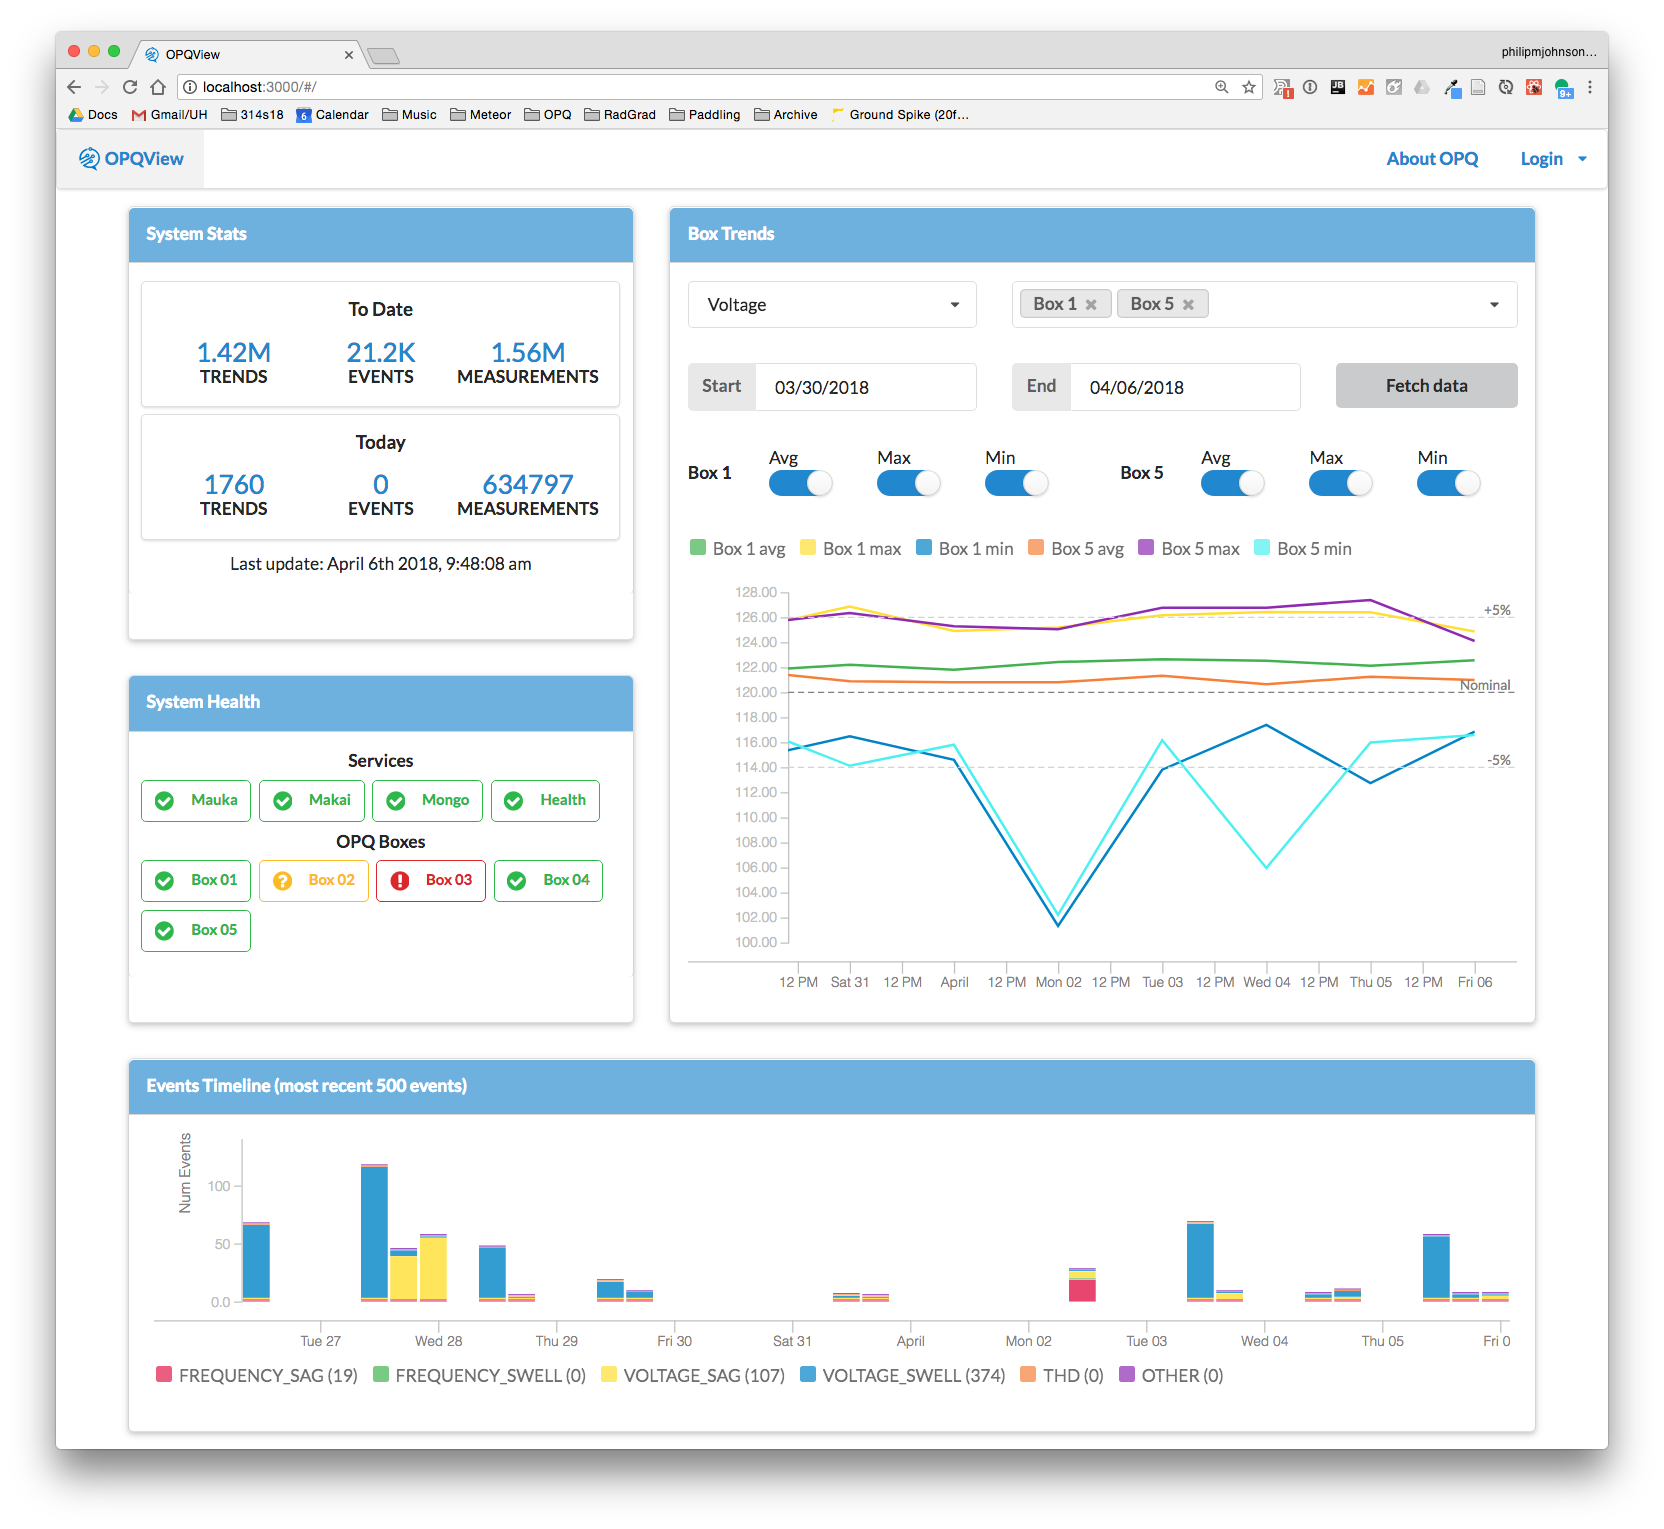
\includegraphics[width=1\linewidth]{figures/opqview-landing-page.png}
	\caption{OPQ View Screenshot}\label{fig:opq-view}
\end{figure}



\subsection{OPQ: Data Model}
TODO

\subsection{OPQ: Dockerfication}
TODO

%\subsection{OPQ as a Laha-compliant DSN}
%OPQ and specifically OPQMauka comply with the Laha abstract framework. Table \ref{opq-compliance} summarizes how the OPQ data architecture fits within the Laha conceptual model.
%
%\begin{table}
%	\caption{OPQ as a Laha-compliant DSN}
%	\begin{tabular}{|c|c|c|c|c|}
%		\hline 
%		Laha Level & OPQ & Created By & Stored By & TTL \\ 
%		\hline 
%		IML & raw ADC Samples & OPQBox & Onboard memory & 20 minutes \\ 
%		\hline 
%		AML & min,max,avg V, F, THD & OPQBox & trends\footnotemark & 1 day \\ 
%		\hline 	
%		DL & triggered waveforms & Makai/Mauka & events/box\_events\textsuperscript{\ref{fn-1}} & 1 week \\
%		\hline
%		IL & Classified detections & Mauka & incidents\textsuperscript{\ref{fn-1}} & 1 year \\
%		\hline
%		PL & Predictive analytics & Mauka & phenomena\textsuperscript{\ref{fn-1}} & N/A \\
%		\hline
%	\end{tabular}
%	\label{opq-compliance}
%\end{table}  
%\footnotetext{MongoDB Collection Name\label{fn-1}}
%
%In order to be a Laha compliant DSN, the reference DSN must also implement Laha Actors. Table \ref{opq-actors} summarizes how OPQ implements Laha actors.
%
%\begin{table}
%	\caption{OPQ  Actors Implementation}
%	\begin{tabular}{|c|c|c|}
%		\hline 
%		Laha Actors & OPQ Equivalent & Description \\ 
%		\hline
%		IML Actors & Boxes & Store window of raw sensor samples \\
%		\hline
%		AML Actors & Boxes \& Makai & Makai stores and triggers on aggregate data from Boxes \\
%		\hline
%		DL Actors & Mauka & MakaiEvent plugin \\
%		\hline
%		IL Actors & Mauka & Voltage, Frequency, THD, Outage, plugins \\
%		\hline
%		PL Actors & Mauka & Annotations, Locality, Similarity,  Periodic, Predictive,  Future plugins\\
%		\hline
%	\end{tabular}
%	\label{opq-actors}
%\end{table}  

\section{Lokahi: A Laha-compliant Infrasound DSN}
Lokahi is a dynamic DSN that originally evolved as a distributed infrasound detection network. Infrasound is characterized as sound waves that are less than 20 Hz. Infrasound generally can not be deciphered by the human ear, but it can be detected using microphone and barometric pressure sensors. Any large movements of the atmosphere can produce infrasound. The Lokahi network was designed to supplement the International Monitoring System (IMS) for the capture  of undeclared and declared nuclear explosions. Lokahi has been successfully used to capture signals from volcanoes, hurricanes, aircraft, meteors, and other large atmospheric events. 

Sensors in Lokahi are any mobile device that can run iOS or Android. We have sensors distributed world wide. The software stack for Lokahi consists of a distributed actor system for data acquisition, MongoDB for metadata persistence, Apache Kafka for data queues and interprocess communication, Python and related scientific libraries for analysis, and a distributed key-value store for long term storage or sensor data.

Recent development and improvements to the data API have allowed Lokahi to begin accepting data from any of the available onboard sensors on iOS and Android devices. Even though the main focus is still infrasound, having access to all of the available sensors provides the ability to sense other sensor fields and to perform interesting data fusion techniques. 

A diagram of the Lokahi framework is provided in figure \ref{fig:lokahi}.


\begin{figure}
	\centering
	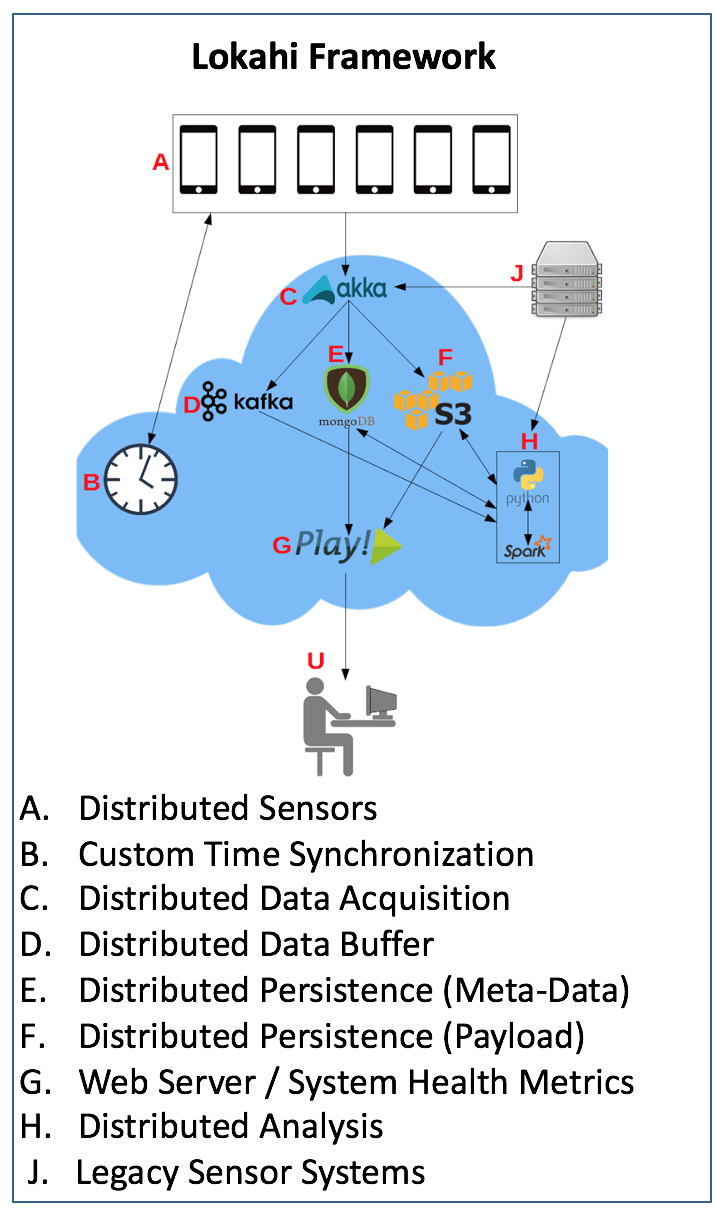
\includegraphics[]{figures/lokahi.png}
	\caption{Lokahi Design}\label{fig:lokahi}
\end{figure}

%\subsubsection{Lokahi: Ingestion}
%Unlike OPQ, Lokahi takes an approach of send and store everything from every sensor, all the time. This approach is vastly different than what we're used to in triggering based acquisition systems. Data between sensors and our Ingestion servers is encrypted using standard SSL encryption algorithms. Authentication and authorization for each sensor is accomplished using Json Web Tokens (JWTs) with signatures generated using elliptic curve cryptography (ECC). Data at the sensor level is serialized using protocol buffers and then compressed using LZ4. 
%
%To enable the smooth retrieval of large amounts of sensor data, Lokahi uses a distributed actor system (Akka) to automatically scale horizontally based on the current volume of data being received. 
%
%\subsubsection{Lokahi: Persistence}
%Metadata is stripped from the sensor data at data ingestion and immediate stored to a distributed Mongo database. Metadata is indexed using a combination of device id and timestamps. 
%
%Metadata drives the rest of the Lokahi framework and provides pointers to the raw data.
%
%Raw sensor data is stored in a distributed key-value store. Lokahi uses Amazon's Simple Storage Service (S3) which provides automatic data redundancy and essentially limitless storage. Raw sensor data is stored by key and the key is stored in the metadata.
%
%Raw sensor data is also persisted in an Apache Kafka queue. Kafka not only provides the framework with a message queue to pass data between distributed services, but it also acts as a ring buffer. Each sensor stores 1 hours worth of data in Kafka that can be looked up by any of the distributed clients and retrieved very quickly. For those reasons, Kafka powers IPC and data buffering roles for our real time analysis of Lokahi sensor data streams.  
%
%\subsubsection{Lokahi: Analysis}
%Analysis in Lokahi is provided by a set of distributed processes that were developed in Python using SciPy, NumPy, and matplotlib. Recent developments in the framework are now also including the basis for machine learning (ML) using Tensor Flow.
%
%We provide real time plotting and analysis by subscribing to real time data feeds provided by the Apache Kafka real time queue and buffer. We also provide more robust batch analysis of historical data that can be initiated from Lokahi Web.
%
%
%\subsubsection{Lokahi: Web}
%Lokahi web is a web application for querying and performing analysis of real time sensor data or over historical sensor data. Lokahi also has built in system of health displays for providing a real-time and historic overview of the health of the distributed services within the framework. 
%
%% TODO, provide screenshot

%\subsubsection{Lokahi as a Laha-compliant DSN}
%TODO